
\documentclass[journal]{IEEEtran}
\usepackage{cite}
\usepackage[utf8]{inputenc}
\usepackage[T1]{fontenc}
\usepackage{caption}
\usepackage{url}
\usepackage{amssymb}
\usepackage{amsmath}
\usepackage{algorithm}
\usepackage{graphicx}
\graphicspath{ {images/} }

% correct bad hyphenation here
\hyphenation{op-tical net-works semi-conduc-tor}


\begin{document}


% paper title
\title{Review of procedural content generation methods and applications}

% author names and IEEE memberships
\author{
Bojan Lovrovic\\
\textit{Faculty of Electrical Engineering and Computing}\\
\textit{University of Zagreb}\\
\textit{Zagreb, Hrvatska}

\thanks{}
}

% make the title area
\maketitle

\section{Uvod}
\IEEEPARstart{V}{}eć pri prvim primjenama računala za igranje igara -- štoviše, čak i
prije nego su te programe mogli upogoniti na računalima -- ljudi su bavili
problematikom igranja šaha.

Za igranje šaha, postoje dva glavna pristupa:
 - brute-force (glupo pretraživanje prostora stanja) uz minimax algoritam, i
 - korištenje heurističkih pravila.
Niti jedan od dva pristupa ne radi dobro sam za sebe, tako da se u pravilu
koristi kombinacija obadva.
"Klasični" program za igranje šaha izgleda otprilike ovako: za početak
se koristi knjiga poteza za otvaranje; nakon početka, koristi se što se
već koristi; za kraj, koristi se unaprijed izračunat endgame tablebase.
Na taj način se pri kraju i početku igre igraju sigurno optimalni potezi,
dok je prostor za AI zapravo u središnjem dijelu igre.

Osnovni algoritam za šah (i druge turn-based igre) je minimax algoritam.
Ideja iza algoritma je sljedeća: dva racionalna igrača igraju jedan protiv
drugog. Uz nekakvu mjeru dobrote -- koliko je stanje dobro za prvog igrača
-- prvi igrač tu mjeru želi maksimizirati, a drugi je minimizirati. Svaki
igrač igra onaj potez koji ga najviše približava tom cilju, odnosno prvi
igrač odabire potez najveće mjere dobrote, a drugi najmanje.

Prostor stanja možemo zamisliti kao stablo: početno stanje je korijen,
dozvoljena sljedeća stanja su njegova djeca, a prijelaz iz jednog stanja
u drugo odgovara odabiru jednog djeteta/podstabla.

Algoritam pretražuje prostor stanja tako da simulira sve moguće igre
krenuvši iz početnog stanja, odnosno pretražuje sve grane stabla.
Pritom svaki "sloj" (skup svih čvorova na nekoj dubini, engl. ply) odgovara
stanju gdje je jedan od igrača na potezu. U korijenu, taj igrač je
maksimizator (MAX, odnosno "mi") -- on za najbolji potez odabire dijete s
najvećom dobrotom; u sloju odmah ispod (na dubini 1), igrač je minimizator
(MIN, odnosno "neprijatelj") -- on za (svoj) najbolji potez odabire dijete s
najmanjom dobrotom; u sloju ispod tog (na dubini 2), igrač je opet MAX, i t.d.

Svaki od igrača zapravo nastoji minimizirati svoj maksimalni mogući gubitak.
Tako je najbolji potez maksimizatora maksimum od minumuma maksimumâ ...
Hence the name, minimax.

Ako nema više potezâ, znači da je dostignut mat ili remi, i dobrota tog stanja
se definira kao +1 (pobjeda), -1 (gubitak), ili 0 (izjednačeno). S obzirom da
u pravilu ne možemo pretražiti *cijelo* stablo, nakon neke zadane dubine se za
evaluaciju dobrote stanja koristi neka heuristika.

\iffalse
Pseudokôd:
```
funkcija minimax( ploča, igrač, dubina ):
    
    legalni_potezi <- generiraj_moguće_poteze( ploča )

    ako dubina == 0 ili !legalni_potezi:
        vrati heuristička_evaluacija( ploča, igrač )

    inače, za svaki legalan potez:
        hipotetska_ploča <- odigraj( ploča, potez )
        dobrota <- minimax( hipotetska_ploča, ~igrač, dubina-1 )
        zapamti dobrotu
    
    ako igrač == MAX:
        najbolji_potez <- potez najveće dobrote
    inače:
        najbolji_potez <- potez najmanje dobrote

    vrati najbolji_potez
```
\fi

\section{Pregled područja}
Šah spada u veliku skupinu društvenih igara koje je relativno jednostavno naučiti ali zahtjevno za izvještiti. Drugim riječima, pravila igre su, matematički gledano, dobro definirana, pa je implementacija šaha na računalu predmet proučavanja dugi niz godina. Od 1950-tih razvijeno je stotine različitih programskih rješenja igranja šaha. Uobičajena formulacija problema jest za zadanu trenutačnu konfiguraciju vlastitih i protivničkih figura na ploči, odabrati jedan od dozvoljenih poteza kojim se maksimizira vjerojatnost pobjede. U svrhu spomenutog, prirodno je protivnika modelirati na isti način, pretpostavljajući da će i on vuči poteze koristeći isti mehanizam kao i mi (teorija igara).

U duhu principa korištenih u umjetnoj inteligenciji, današnja \textit{eng. state-of-art} programska rješenja ovog problema temelje se na pretraživanju prostora stanja modeliranih stablima pretraživanja. Svaka razina ovog stabla sadrži sve poteze koje igrač koji je na redu smije povući. Čvorovi u zadnjoj razini stabla nazivaju se listovi i njima je s obzirom na ishod partije pridijeljena odgovarajuća ocjena (1, -1 ili 0 u slučaju neriješenog ishoda). Iako bi teoretski mogli u svakom čvoru čuvati sumu ocjene listova do kojih taj čvor vodi i tako u svakom trenutku imati stvarnu ocjenu čvora, u praksi je takvo pridjeljivanje nemoguće izračunati u stvarnom vremenu. Razlog tome je broj mogućih poteza koji raste eksponencijalno nakon svakog odigranog poteza. Umjetna inteligencija ovom problemu doskače podrezivanjem stabala na unaprijed određenoj razini D, tako da se daljnje razine ni ne razmatraju, već se koristi ocjena čvorova te razine dodijeljena funkcijom evaluacije. Ispostavlja se da je implementacija ove funkcije jedan od najbitnijih segmenata u modeliranju sustava a naša zamisao bila je prepustiti aproksimiranje evaluacijske funkcije neuronskoj mreži.

Ideja je iz poznatih odigranih partija izvući veliku količinu konfiguracija, opisati ih značajkama i onda, korištenjem trenutno najpopularnijeg \textit{eng. chess engine}-a Stockfish, svakoj mogućoj konfiguraciji dodijeliti ocjenu na način da bolja ocjena odgovara većoj vjerojatnosti konačne pobijede. Na tako generiranom skupu podataka učimo neuronsku mrežu koju kasnije, tijekom igre, koristimo za procjenu ocjene određenog poteza.

Šah je između ostalog i \textit{eng.zero-sum} igra što znači da suma svih ocjena teži prema nuli. U skladu s tim, pozitivna ocjena jednom igraču, negativna je za drugog, i obrnuto. Sad je lako za uočiti kako se prvobitni problem svodi na izbor poteza kojim se minimizira protivnikova pobjeda (i samim time maksimizira vlastita), odnosno bira se potez s najlošijom ocjenom za protivnika.

Spomenutim principom vode se poznatija suvremena rješenja zasnovana na strojnom učenju, pa i radovi Erika Bernhardssona te Matthewa Laija, na kojem se temelji naš rad.

Učenjem funkcije koja ocjenjuje svaku konfiguraciju ploče i kombiniranjem s algoritmom pretraživanja stanja možemo napraviti stroj koji igra šah. Erik Bernhardsson je ponudio rješenje u kojem je iz velikog skupa igara naučio funkciju evaluacije poteza preko trenutnog poteza p, sljedećeg poteza q i nasumično odabranog poteza r. Funkcija koju uči pretpostavlja da je sljedeći odabran potez q blizu optimalnog, a nasumično odabrani potez r gori od poteza q. Takva funkcija ne ovisi o pravilima šaha, što znači da njegova mreža mora iz skupa igara moći naučiti što su legalni potezi i kako se figure pomiču. Mreža se sastoji od 3 sloja i na ulaz prima 8*8*12 vrijednosti koje predstavljaju ploču i figure na ploči. Nakon naučene funkcije evaluacije za igranje šaha koristi negamax pretraživanje stanja s alfa-beta odsijecanjem.

Možda glavni problem kod prije spomenute metode je reprezentacija ulaza. Konfiguracije ploče sa sličnom evaluacijom bi trebale biti međusobno blizu u ulaznom prostoru. Rješenje Matthewa Laija iz svake konfiguracije izvlači više informacije od same pozicije figura. Rezultat je prostor značajki od oko 360 značajki za svaku konfiguraciju koje uzimaju u obzir koje su figure napadnute, koje obranjene, prava na rokadu te koliko daleko klizeće figure mogu ići, među ostalima. Navedene značajke čine prostor značajki gdje se slične situacije u igri nalaze međusobno blizu u ulaznom prostoru. Na temelju ovakvih značajki duboka neuronska mreža može naučiti složenije koncepte i skrivena znanja u igri šaha bez potrebe za implementiranjem složenijih pravila, te se smanjuje potreba za dubljim pretraživanjem prostora stanja prilikom odluke.

Njegova evaluacijska funkcija koristi prilagođenu verziju TD-Leaf algoritma koja procjenu ne temelji na ishodu partije već na odlukama koje bi ista funkcija donijela u nekom potezu u bliskoj budućnosti. Također, dio stabla koji se uzima u obzir kod pretraživanja nije određen dubinom kao kod većine današnjih sličnih sustava, već vjerojatnošću da odabrana staza u stablu bude dio teoretski optimalne staze koja vodi do kraja partije uzimajući u obzir da se oba igrača vode istom logikom igranja.





\section{Implementacija}
Implementacija se temelji na diplomskom projektu studenta Matthewa Laija \cite{giraffe}. Ovo poglavlje će proći kroz postupak generiranja skupa za učenje, izvlačenje vektora značajki za pojedini ulazni primjer, izradu te na kraju treniranje mreže.
\subsection{Generiranje podataka za učenje}
Prije svega potrebno je bilo generirati skup podataka za učenje. Pri tome se je koristila baza igara gdje je za svaku igru bila poznata lista poteza. Iz ove liste je dobivene lista stanja kroz cijelu igru te je svakom stanju pridružena ocijena dobivena evaluacijom. Iako je \cite{giraffe} rađen uz pomoć vlastite evaluacijske funkcije, mi smo koristili Stockfish. Lista parova stanja i ocjene u konačnici čini naš skup primjera za učenje.
\subsection{Vektor značajki}
Izvlačenje vektora značajki se dijeli na tri grupe: globalne značajke, značajke vezane uz figure te značajke vezane uz kvadrate. Valja napomenuti da iako pojedini elementi ovoga vektora poprimaju vrijednosti iz različitih domena, na kraju izvlačenja ove su vrijednosti transformirane u domenu $\left[0,1\right]$.
\par
Globalne značajke započinju sa binarnom vrijednosti koja predstavlja informaciju jeli bijeli na redu. Slijede četiri skalara od kojih je svaki zastavica sa vrijednosti postavljenom na jedan ukoliko je trenutačno omogućena ta rošada. Posljednji u listi globalnih značajki je podvektor kod kojeg je svaki element broj trenutno prisutnih figura na ploči za pojedini tip figure.
\par
Značajke vezane uz figure su sastavljene od liste figura sa lokacijama i ostalim podatcima potrebnim ovisno o tipu figure. Za reprezentaciju ploče bilo je potrebno koristiti \textit{python chess} koji u sebi nema mehanizam diskriminacije različitih figura istog tipa, dok je u \cite{giraffe} takvo svojstvo navedeno kao obavezno. To je bio glavni razlog za izradu našeg sučelja za kontrolu stanja ploče, izgrađenog povrh već postojećeg \textit{python chessa}. Naše sučelje sprema poziciju svake figure te ju ažurira prilikom svakog pokreta jednog od igrača, tako da se one mogu međusobno razlikovati. Ovo u praksi znači da će informacije o ljevom lovcu uvijek stizati na istom mijestu u vektoru značajki bez obzira gdje se on na ploči nalazio (čak i ako si lijevi i desni lovac zamijene lokacije). Uz lokaciju, za neke je figure potrebno poslati još i dozvoljeno klizanje u bilo kojem dozvoljenom smjeru. Ovdje se konkretno radi o četiri broja za kulu i lovca, te osam za kraljicu, budući da ona može klizati u osam smjerova.
\par
Značajke vezane uz kvadrate imaju ocjenu najslabijeg napadača i najslabijeg branitelja za pojedino polje i te su dvije vrijednosti prisutne za svaki kvadrat (polje) na ploči. Vrijednosti pojedinog tipa figure dane su u tablici \ref{tab:vrijednosti}.
\begin{table}[]
\centering
\captionof{table}{Vrijednosti figura.}
\label{tab:vrijednosti}
\begin{tabular}{lc}
\textbf{Figura} & \multicolumn{1}{l}{\textbf{Vrijednost}} \\ \hline
Pijun           & 1                                       \\
Konj            & 3                                       \\
Lovac           & 3                                       \\
Kula            & 5                                       \\
Kraljica        & 9                                       \\
Kralj           & 15                                     
\end{tabular}
\end{table}
\subsection{Izrada mreže}
Topologija mreže se sastoji od dva skrivena sloja te jednog izlaznog kao na slici \ref{fig:topologija}. Ulazni sloj je sa prvim skrivenim povezan lokalno, dok su prvi i drugi skriveni povezani potpuno. Drugi skriveni sloj je sa izlaznim slojem odnosno neuronom također povezan potpuno. Brojevi neurona po slojevima mreže mogu se vidjeti u tablici \ref{tab:brneurona}.
\begin{figure}[H]
	\centering
	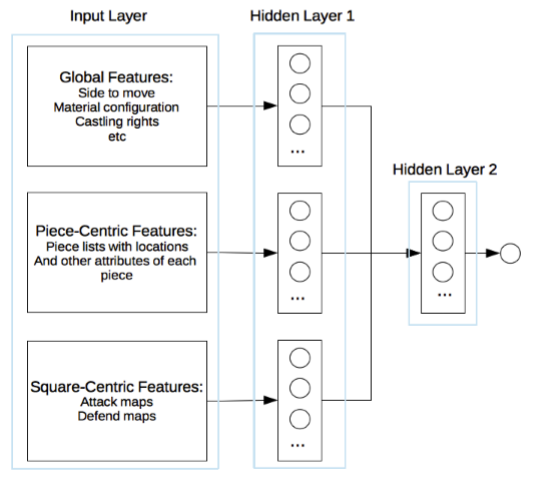
\includegraphics[width=.8\linewidth]{networkArchitecture.png}
	\captionof{figure}{Topologija mreže.}
	\label{fig:topologija}
\end{figure}
\begin{table}[]
\centering
\captionof{table}{Broj neurona po slojevima.}
\label{tab:brneurona}
\begin{tabular}{lc}
\textbf{Sloj} & \multicolumn{1}{l}{\textbf{Broj neurona}} \\ \hline
Ulazni (prvi dio)           	& 15		\\
Ulazni (drugi dio)		& 144		\\
Ulazni (treći dio)		& 128		\\
Prvi skriveni (prvi dio)	& 10		\\
Prvi skriveni (drugi dio)	& 110		\\
Prvi skriveni (treći dio)	& 100		\\
Drugi skriveni		& 100		\\
Izlazni				& 1		\\                    
\end{tabular}
\end{table}


\subsection{Treniranje mreže}
Ovdje napisi nes Zlatane!!!! :)



\section{Zaključak}
Although PCG is present for decades, it is still an approach being researched and with it's use rising. Increases in hardware capabilities also have a positive effect on this trend. On the other hand, there is a popular belief that PCG can never produce content as good as the artists or designers can. This is definitely true with today's hardware and software capabilities, so the question that poses itself is, where to draw the line. To what point should content be generated and then left out to professionals to do the rest. The approach of no Man's Sky, where almost everything is procedurally generated, seems too excessive, yet on the contrast, generating random noise in image editor pixel by pixel would be even worse. Whenever the line might be, it will surely move in avail of PCG and we are yet to see much more surprises from this field.

% Can use something like this to put references on a page
% by themselves when using endfloat and the captionsoff option.
\ifCLASSOPTIONcaptionsoff
  \newpage
\fi

\bibliographystyle{plain}
\bibliography{references}

\end{document}


